\documentclass{sigchi}

% Use this section to set the ACM copyright statement (e.g. for
% preprints).  Consult the conference website for the camera-ready
% copyright statement.

% Copyright
%\CopyrightYear{2020}
%\setcopyright{acmcopyright}
%\setcopyright{acmlicensed}
%\setcopyright{rightsretained}
%\setcopyright{usgov}
%\setcopyright{usgovmixed}
%\setcopyright{cagov}
%\setcopyright{cagovmixed}
% DOI
%\doi{https://doi.org/10.1145/3313831.XXXXXXX}
% ISBN
% \isbn{978-1-4503-6708-0/20/04}
%Conference
\conferenceinfo{CHI'20,}{November  16--17, 2023, Gatlinburg, TN, USA}
%Price

% Use this command to override the default ACM copyright statement
% (e.g. for preprints).  Consult the conference website for the
% camera-ready copyright statement.

%% HOW TO OVERRIDE THE DEFAULT COPYRIGHT STRIP --
%% Please note you need to make sure the copy for your specific
%% license is used here!
% \toappear{
% Permission to make digital or hard copies of all or part of this work
% for personal or classroom use is granted without fee provided that
% copies are not made or distributed for profit or commercial advantage
% and that copies bear this notice and the full citation on the first
% page. Copyrights for components of this work owned by others than ACM
% must be honored. Abstracting with credit is permitted. To copy
% otherwise, or republish, to post on servers or to redistribute to
% lists, requires prior specific permission and/or a fee. Request
% permissions from \href{mailto:Permissions@acm.org}{Permissions@acm.org}. \\
% \emph{CHI '16},  May 07--12, 2016, San Jose, CA, USA \\
% ACM xxx-x-xxxx-xxxx-x/xx/xx\ldots \$15.00 \\
% DOI: \url{http://dx.doi.org/xx.xxxx/xxxxxxx.xxxxxxx}
% }

% Arabic page numbers for submission.  Remove this line to eliminate
% page numbers for the camera ready copy
% \pagenumbering{arabic}

% Load basic packages
\usepackage{balance}       % to better equalize the last page
\usepackage{graphics}      % for EPS, load graphicx instead 
\usepackage[T1]{fontenc}   % for umlauts and other diaeresis
\usepackage{txfonts}
\usepackage{mathptmx}
\usepackage[pdflang={en-US},pdftex]{hyperref}
\usepackage{color}
\usepackage{booktabs}
\usepackage{textcomp}
\usepackage{float}


% Some optional stuff you might like/need.
\usepackage{microtype}        % Improved Tracking and Kerning
% \usepackage[all]{hypcap}    % Fixes bug in hyperref caption linking
\usepackage{ccicons}          % Cite your images correctly!
% \usepackage[utf8]{inputenc} % for a UTF8 editor only
\usepackage{biblatex} % Imports bibliography stuff

% If you want to use todo notes, marginpars etc. during creation of
% your draft document, you have to enable the "chi_draft" option for
% the document class. To do this, change the very first line to:
% "\documentclass[chi_draft]{sigchi}". You can then place todo notes
% by using the "\todo{...}"  command. Make sure to disable the draft
% option again before submitting your final document.
\usepackage{todonotes}

% Paper metadata (use plain text, for PDF inclusion and later
% re-using, if desired).  Use \emtpyauthor when submitting for review
% so you remain anonymous.
\def\plaintitle{Gardener's Best Friend}
\def\plainauthor{First Author, Second Author, Third Author,
  Fourth Author, Fifth Author, Sixth Author}
\def\emptyauthor{}
\def\plainkeywords{Authors' choice; of terms; separated; by
  semicolons; include commas, within terms only; this section is required.}
\def\plaingeneralterms{Documentation, Standardization}

% llt: Define a global style for URLs, rather that the default one
\makeatletter
\def\url@leostyle{%
  \@ifundefined{selectfont}{
    \def\UrlFont{\sf}
  }{
    \def\UrlFont{\small\bf\ttfamily}
  }}
\makeatother
\urlstyle{leo}

% To make various LaTeX processors do the right thing with page size.
\def\pprw{8.5in}
\def\pprh{11in}
\special{papersize=\pprw,\pprh}
\setlength{\paperwidth}{\pprw}
\setlength{\paperheight}{\pprh}
\setlength{\pdfpagewidth}{\pprw}
\setlength{\pdfpageheight}{\pprh}

% Make sure hyperref comes last of your loaded packages, to give it a
% fighting chance of not being over-written, since its job is to
% redefine many LaTeX commands.
\definecolor{linkColor}{RGB}{6,125,233}
\hypersetup{%
  pdftitle={\plaintitle},
% Use \plainauthor for final version.
%  pdfauthor={\plainauthor},
  pdfauthor={\emptyauthor},
  pdfkeywords={\plainkeywords},
  pdfdisplaydoctitle=true, % For Accessibility
  bookmarksnumbered,
  pdfstartview={FitH},
  colorlinks,
  citecolor=black,
  filecolor=black,
  linkcolor=black,
  urlcolor=linkColor,
  breaklinks=true,
  hypertexnames=false
}

% create a shortcut to typeset table headings
% \newcommand\tabhead[1]{\small\textbf{#1}}

\addbibresource{bibliography.bib}
%%\bibliography{bibliography}

% End of preamble. Here it comes the document.
\begin{document}

\title{\plaintitle}

\numberofauthors{4}
\author{%
  \alignauthor{Chase Duclos\\
   % \affaddr{for Submission}\\
    \affaddr{Hollow Rock, Tennessee}\\
    \email{wescducl@ut.utm.edu}}\\
 \alignauthor{Lucy Gauldin\\
   % \affaddr{for Submission}\\
    \affaddr{Martin, Tennessee}\\
    \email{bildgaul@ut.utm.edu}}\\
  \alignauthor{Vrushank Mali\\
    %\affaddr{for Submission}\\
    \affaddr{Martin, Tennessee}\\
    \email{vrujmali@ut.utm.edu}}\\
  \alignauthor{Shakira Perry\\
    %\affaddr{for Submission}\\
    \affaddr{Martin, Tennessee}\\
    \email{shaaperr@ut.utm.edu}}\\
}

\maketitle

\begin{abstract}
Gardener's Best Friend is a mobile android app for people who want to maintain a journal tracking the well-being of their plants. Within this digital journal, gardeners can meticulously record plant-related information, including health status, watering schedules, and sunlight preferences. The primary goal of this app is to help users maintain their plants' schedule, strengthen their connection with their gardens, and enhance their gardening knowledge by capturing progress photos and documenting their plant journey in a personal journal. Gardener's Best Friend aims to enhance the interaction that gardeners have with their plants, providing users with tools to improve the overall wellness of their gardens.

The app offers further information about each of the user's plants, such as its known preferences regarding sunlight exposure retrieved from a comprehensive database. The database should give the user some insight into their plants' specific needs, ensuring that users can optimize their gardens' care routine. The digital journal even employs a notification system, reminding the user when they need to water their plants, based on the user provided watering schedule. In addition to these features, the app utilizes user location and weather conditions to determine if watering is necessary on a particular day. Overall, Gardener's Best Friend intends to cater to the average novice and expert gardeners alike, looking to keep records of their plants while offering guidance on how to take care of them.

\end{abstract}


% Author Keywords
%\keywords{\plainkeywords}



\section{Introduction}

This comprehensive application is designed to offer a diverse array of features, catering to the needs of plant enthusiasts and individuals keen on maintaining a detailed record of their plant care journey. A prominent function within the app is the inclusion of a diary feature, empowering users to document and track various aspects of their plant's health and growth. To ensure seamless data management, the application is equipped with the capability to leverage either local storage or a database for the secure storage of plant-related information.

In order to enhance the visual aspect of the diary entries, the application seamlessly integrates with the device's camera or gallery, providing users with the flexibility to either capture real-time images of their plants or incorporate existing photos into their diary entries. This visual element not only adds a personal touch to the documentation process but also serves as a valuable visual reference for the user's plant care journey.

Among the innovative features currently in the planning phase is the potential integration of the Google API. This exciting addition allows users to capture an image of their plant, send it to the Google API, and receive insightful information, including the scientific name of the plant. This integration not only facilitates educational aspects of plant care but also adds a layer of sophistication to the user experience.

Further enriching the functionality of the application, discussions are underway regarding the incorporation of a calendar system. Users can opt for either the built-in calendar or an internal calendar within the app. This feature is intended to serve as a robust reminder system, prompting users to make diary entries or attend to essential plant care activities such as watering, ensuring a proactive approach to plant maintenance.

Recognizing the significance of environmental factors in plant care, the application explores the integration of location services. By harnessing location data, the app aims to connect with weather forecasting services, providing users with real-time and localized weather information. This feature empowers users to make informed decisions about their plant care routines based on the specific climatic conditions in their geographical area.

In essence, this application goes beyond a mere plant diary, evolving into a comprehensive tool that amalgamates technological advancements and user-friendly features to create a holistic platform for plant enthusiasts, fostering a deeper connection between users and their green companions.

\section{Background}


The reader should have a general understanding of app development and familiarity with Kotlin and Java, so that the report can delve into advanced concepts of Android development. It can focus on intricate aspects of the Android platform, such as its architecture and components. The report may also touch upon the utilization of Android Studio, assuming the reader's comfort with its features and plugins. Advanced user interface (UI) design principles  can be explored, building on the reader's foundational knowledge. Additionally, discussions on frameworks and libraries like Retrofit, Dagger, and Jetpack may be introduced without providing extensive explanations. By tailoring the content to this audience, the report aims to provide insights that go beyond the basics, offering valuable information for developers already well-versed in Android app development.

\section{Requirements for Application Use}
To fully enjoy the features of Gardener's Best Friend, the user's mobile device must meet a few requirements. These requirements exist to enhance the user's overall experience, ensuring that every function implemented works seamlessly.

Firstly, the user's mobile device must at least run on API level 28. This minimum API requirement guarantees compatibility with the technologies integrated into Gardener's Best Friend. If this requirement is met, users can enjoy all the features without any technical limitations. API level 28 and above provide the necessary framework for the app to perform optimally, delivering a smooth and responsive experience.

Secondly, the presence of a functional camera on the mobile device is a crucial requirement for utilizing the app's journaling feature. Gardener's Best Friend relies on the device's camera, allowing users to capture and log the progress of their plants.

Additionally, the mobile device must have a reliable method of storing data for the app's retrieval. This requirement guarantees that the pictures taken by the device's camera can be efficiently saved and accessed by Gardener's Best Friend. Adequate storage capacity is essential for maintaining a comprehensive record of the user's gardening journey.

Lastly, a device with internet access is required to use the Perenual API. The API relies on internet access to retrieve data to present the user with information about the plants they have added to their journal.

By meeting these specified requirements, users can unlock the full potential of Gardener's Best Friend, transforming their mobile devices into digital journals for growing healthy and thriving gardens.

\section{Required Functions}

Our application is designed to cater to the diverse and dynamic needs of plant enthusiasts, requiring a rich set of functionalities to enhance the user experience. Foremost among these features is the ability to effortlessly add and showcase photos, empowering users to visually document the journey and flourishing of their plants. The diary entry function is equally indispensable, serving as a digital journal for users to record detailed observations, growth milestones, and personalized insights, creating a narrative that evolves with each plant's unique story. To ensure optimal and mindful plant care, a fundamental requirement is the integration of a user-friendly watering schedule feature. This feature allows users to set and manage watering routines, ensuring that each plant receives the right amount of hydration at the right times.

Furthermore, our application necessitates the capability to seamlessly query an external API for plant information. This integration provides users with access to a wealth of data, including detailed care guidelines, botanical facts, and insights sourced from the API. This not only empowers users with knowledge but also enriches their understanding of the plants under their care. In essence, these required functionalities collectively form the backbone of our application, creating a holistic and intuitive platform for plant enthusiasts to cultivate a deep connection with their green companions, supported by a wealth of information and features that promote both expertise and joy in the art of plant care.

\section{Technology}
The technological foundation of our cutting-edge plant care application represents a carefully curated ensemble of tools, each contributing distinctive features to ensure a comprehensive, feature-rich, and technologically advanced user experience. At the core of our development efforts is Android Studio, an indispensable integrated development environment (IDE) renowned within the Android app development community. Beyond its user-friendly interface, Android Studio boasts an extensive suite of features that lays a robust foundation for efficient coding, meticulous debugging, and thorough testing, guaranteeing the delivery of a high-caliber application.

In the realm of programming languages, our unwavering commitment to excellence led us to embrace Kotlin, a language endorsed by Google for Android development. Beyond its syntactical elegance, Kotlin introduces a modern and concise coding style that significantly enhances code readability and reduces boilerplate code. The language's seamless interoperability with existing Java code not only facilitates a smooth integration process but also positions our application for long-term scalability and maintainability, ensuring the adaptability of our codebase to evolving needs.


For the crucial task of local data storage, our choice is SQLite, a venerable relational database management system. Acknowledged for its lightweight nature and efficiency in managing structured data, SQLite emerges as an optimal choice for our mobile application. Its reliability in performance ensures swift and secure data storage and retrieval, contributing to a seamless user experience without compromising on the integrity of stored data.

In our relentless pursuit of a dynamic and enriched user experience, the integration of the Perenual API represents a pivotal leap forward. This collaboration elevates our application beyond the confines of a conventional plant diary. Users can now access real-time, in-depth information about their plants, including intricate scientific details. The Perenual API transforms our application into a dynamic hub of plant-related knowledge, positioning it at the forefront of technological innovation in the domain of plant care applications. This dynamic integration not only caters to the informational needs of users but also infuses a layer of sophistication into their plant care journey.

To orchestrate seamless collaboration and foster an agile development process, GitHub takes center stage as our version control and collaboration platform. GitHub's robust suite of tools encompasses version control, issue tracking, and code review features, fostering a collaborative and transparent environment within our development team. This strategic choice not only underscores our commitment to delivering a product but also emphasizes our dedication to continuous improvement and innovation in the realm of plant care applications.

In essence, our extensive technological stack, comprising Android Studio, Kotlin, SQLite, the Perenual API, and GitHub, unfolds as a meticulously selected array of tools. This strategic amalgamation, enriched with robust features, not only empowers our development team but also ensures that our end-users embark on a technologically advanced, seamless, and gratifying plant care journey. In setting new standards for mobile applications catering to plant enthusiasts, we aspire to redefine the landscape with an application that transcends expectations, offering a harmonious blend of functionality and innovation. \newline \newline \newline \newline \newline  \newline 

%\LaTeX\ sometimes will create overfull lines that extend into columns.
%To attempt to combat this, the \texttt{.cls} file has a command,
%\texttt{{\textbackslash}sloppy}, that essentially asks \LaTeX\ to
%prefer underfull lines with extra whitespace.  For more details on
%this, and info on how to control it more finely, check out
%{\url{http://www.economics.utoronto.ca/osborne/latex/PMAKEUP.HTM}}.


\section{Mockups}
In the beginning stages of developing Gardener's Best Friend, we started the design process with the creation of mockups. These mockups served as a starting point for our user interface.

\begin{figure}[H]
    \centering
    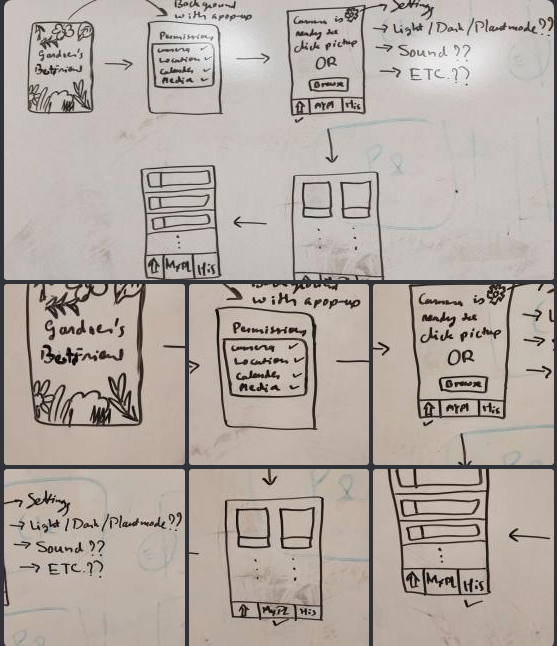
\includegraphics[width=2.5cm, height=4cm]{OldMockup}
	\\\emph{Figure 1.} Initial mockup drawings on whiteboard.
\end{figure}

\begin{figure}[H]
    \centering
    
\includegraphics[width=2.5cm, height=4cm]{Load Screen}
    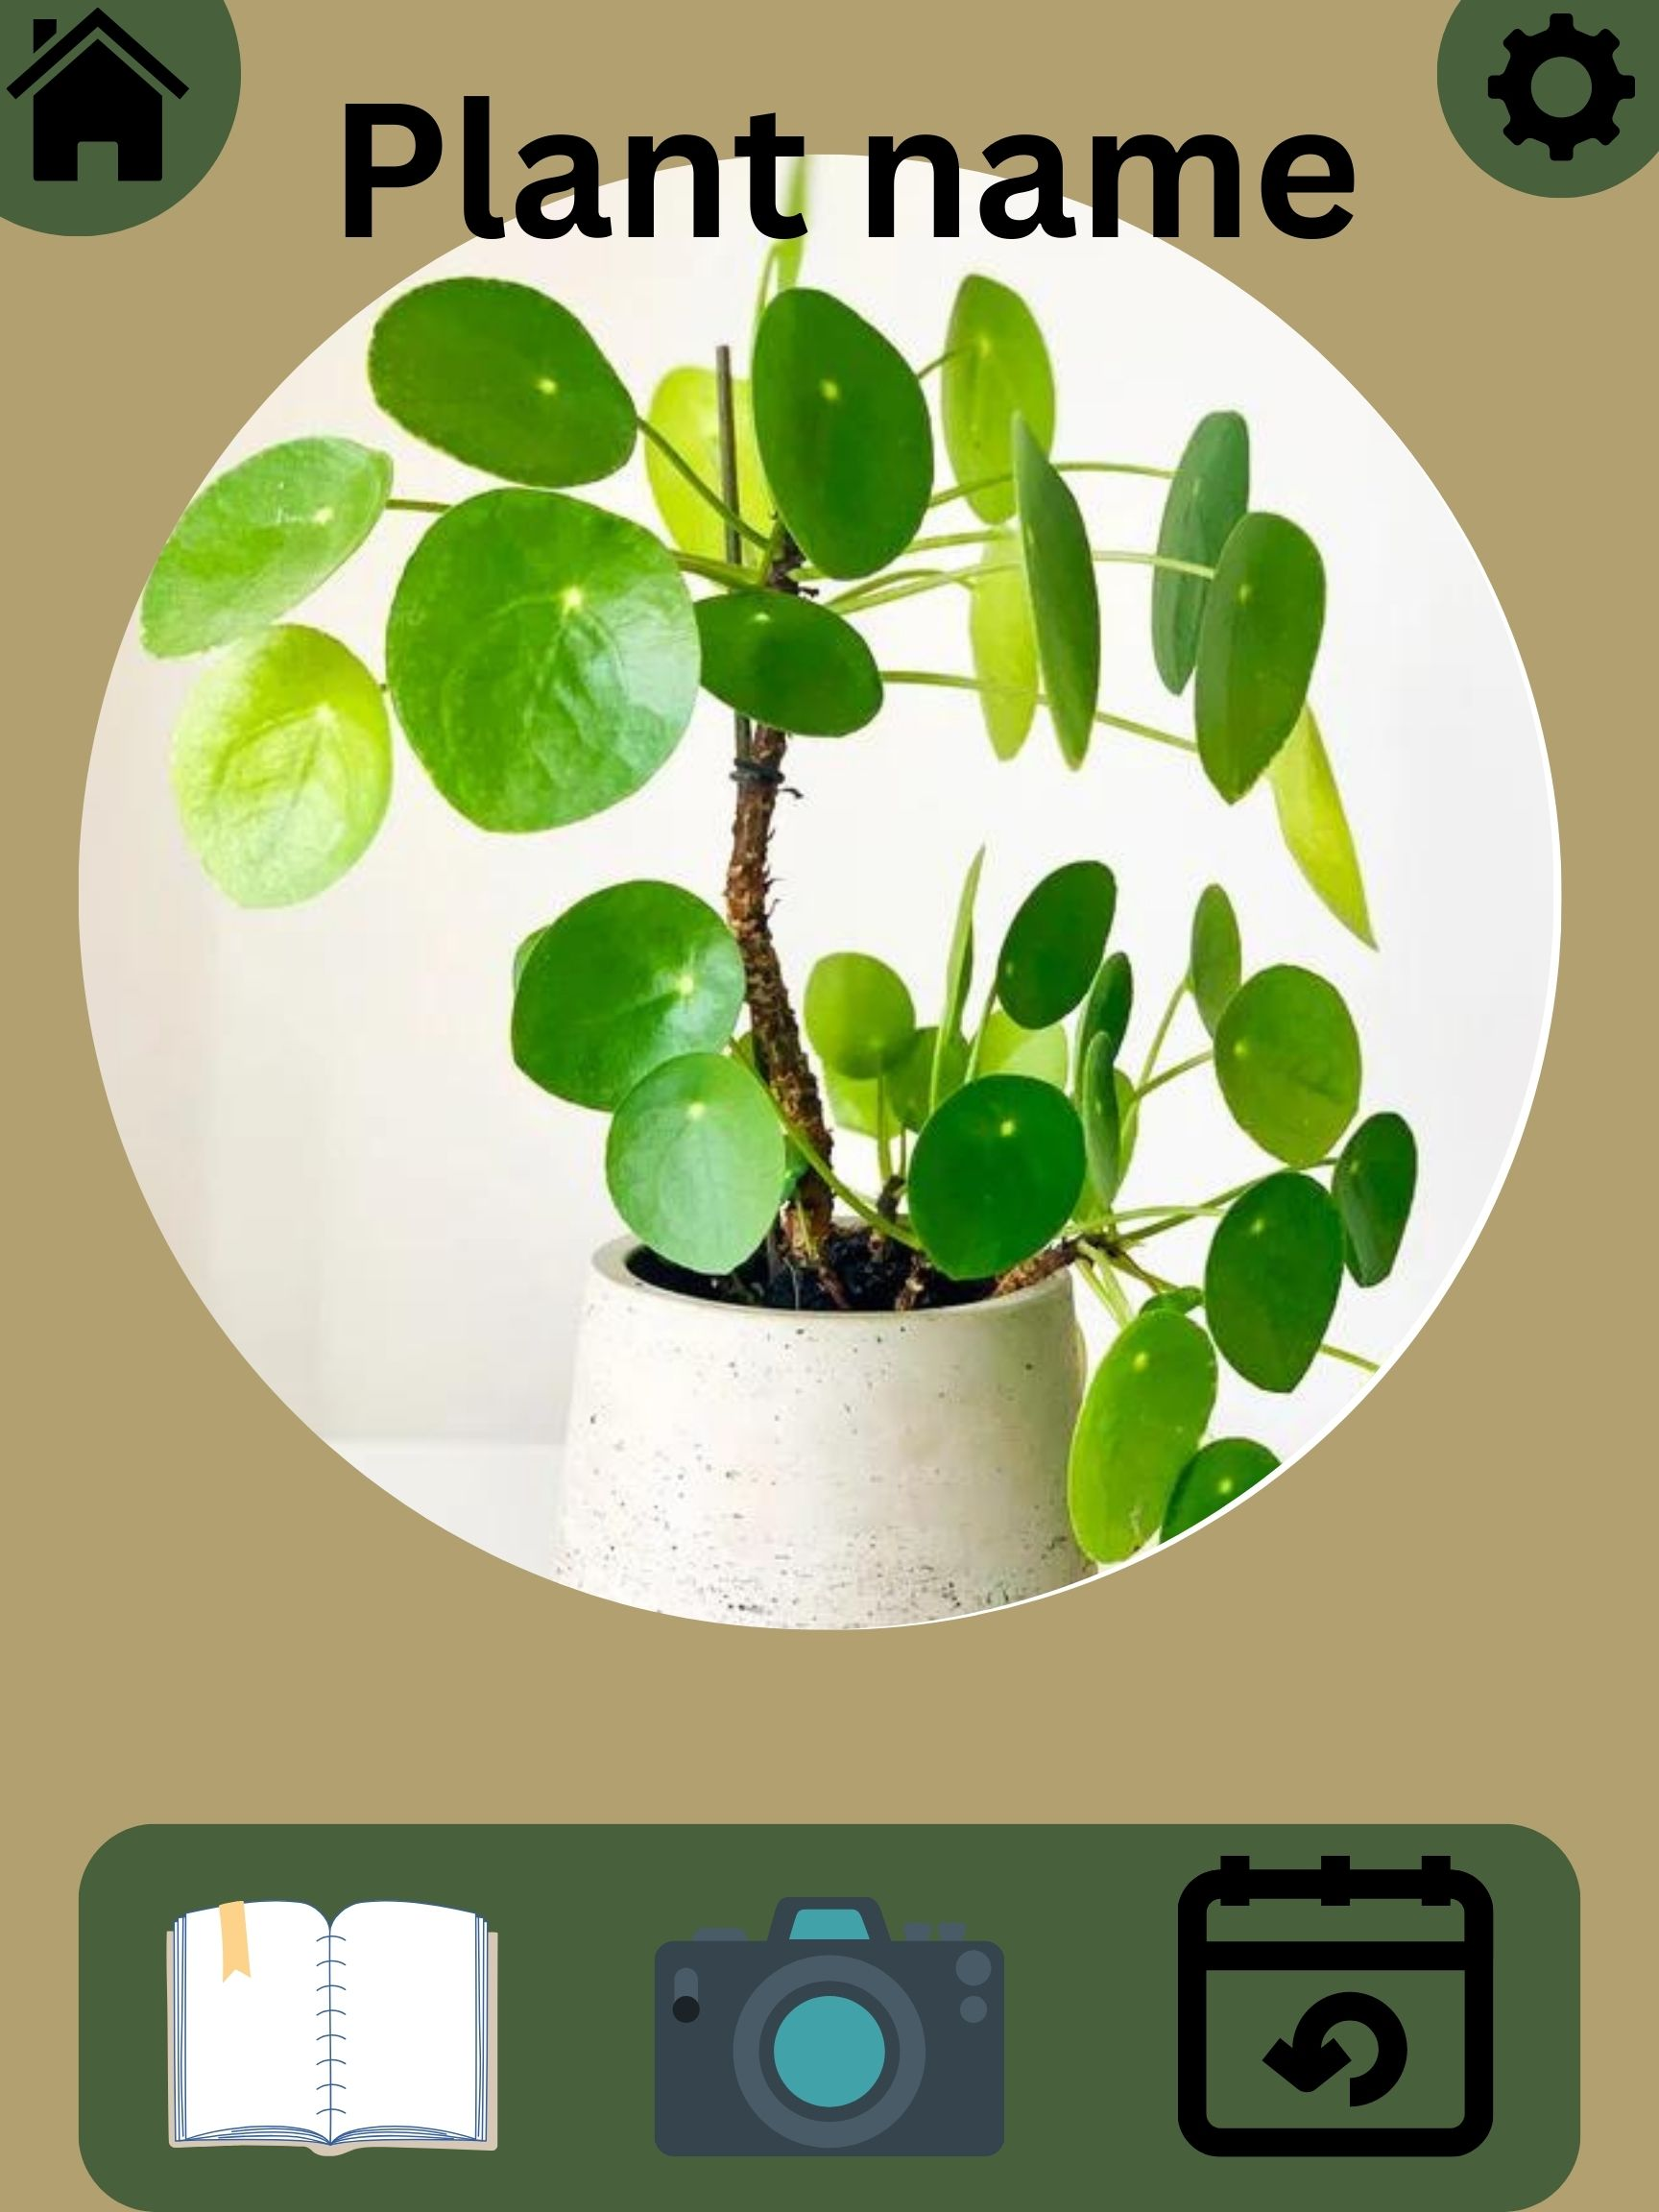
\includegraphics[width=2.5cm, height=4cm]{HomePlantAdded}
	\\\emph{Figure 2-3.} Splash Screen and home page after plant added.
\end{figure}

\begin{figure}[H]
    \centering
    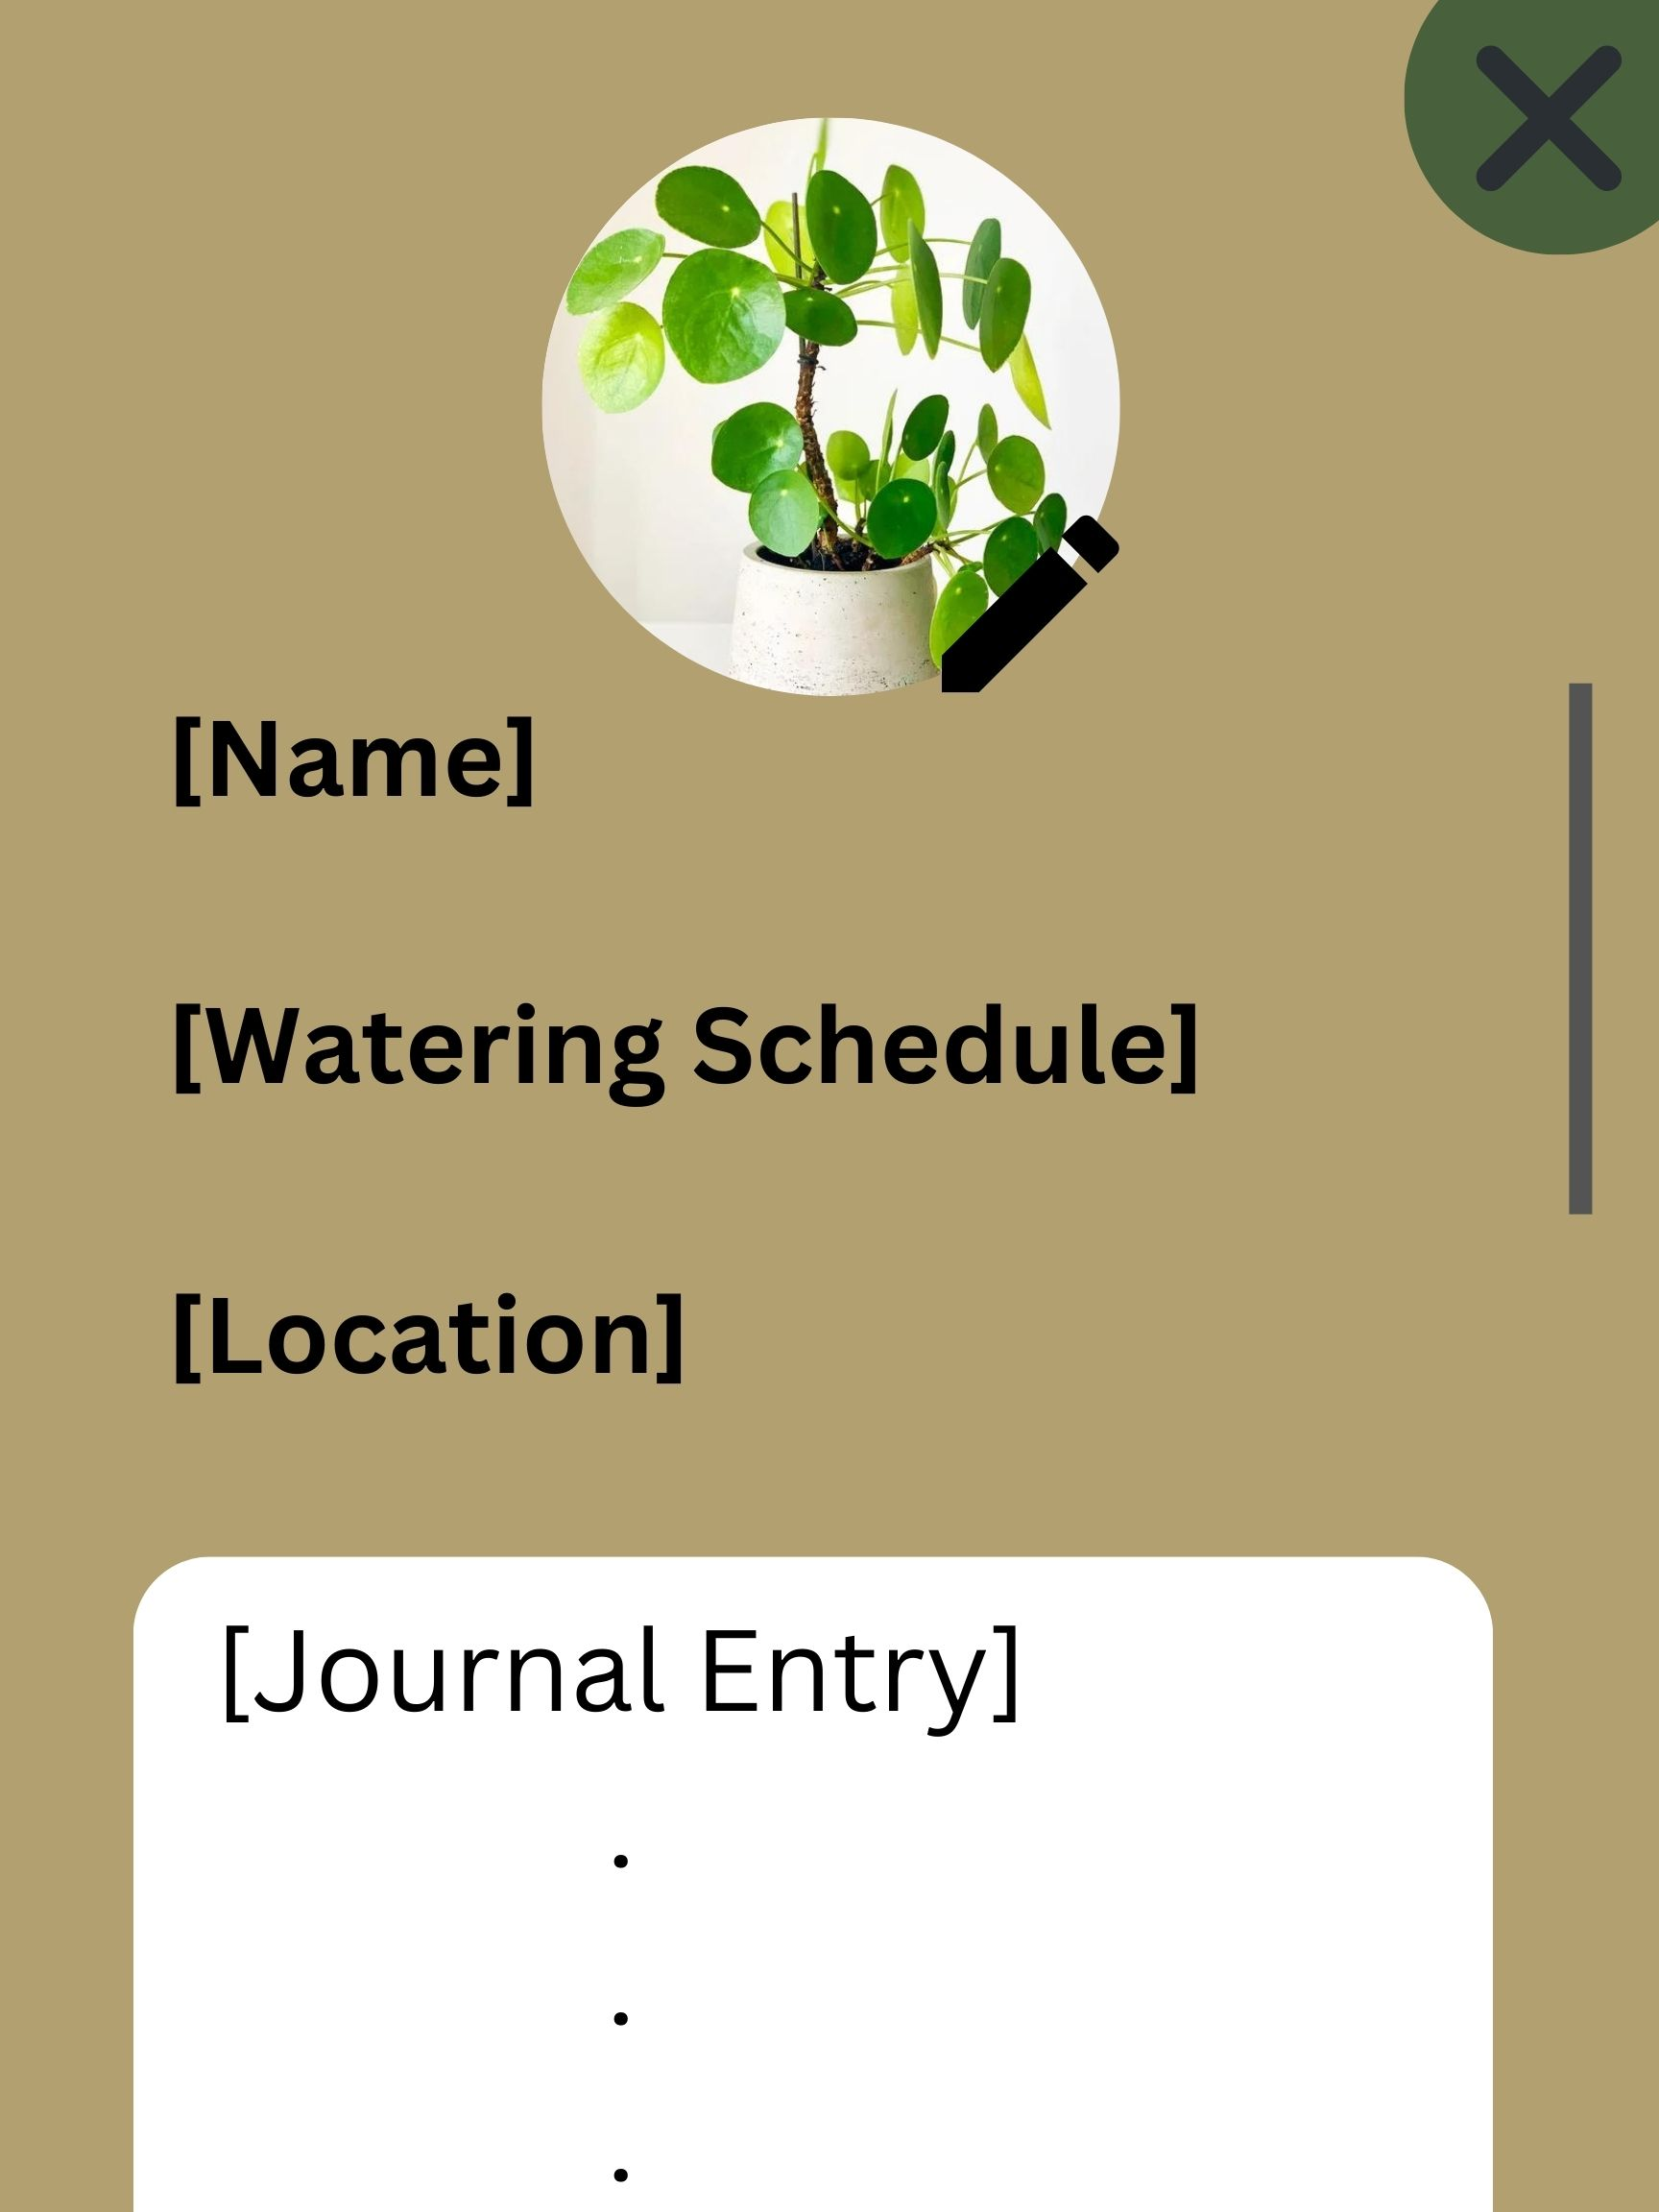
\includegraphics[width=2.5cm, height=4cm]{NewPlantOrEditExisting}
    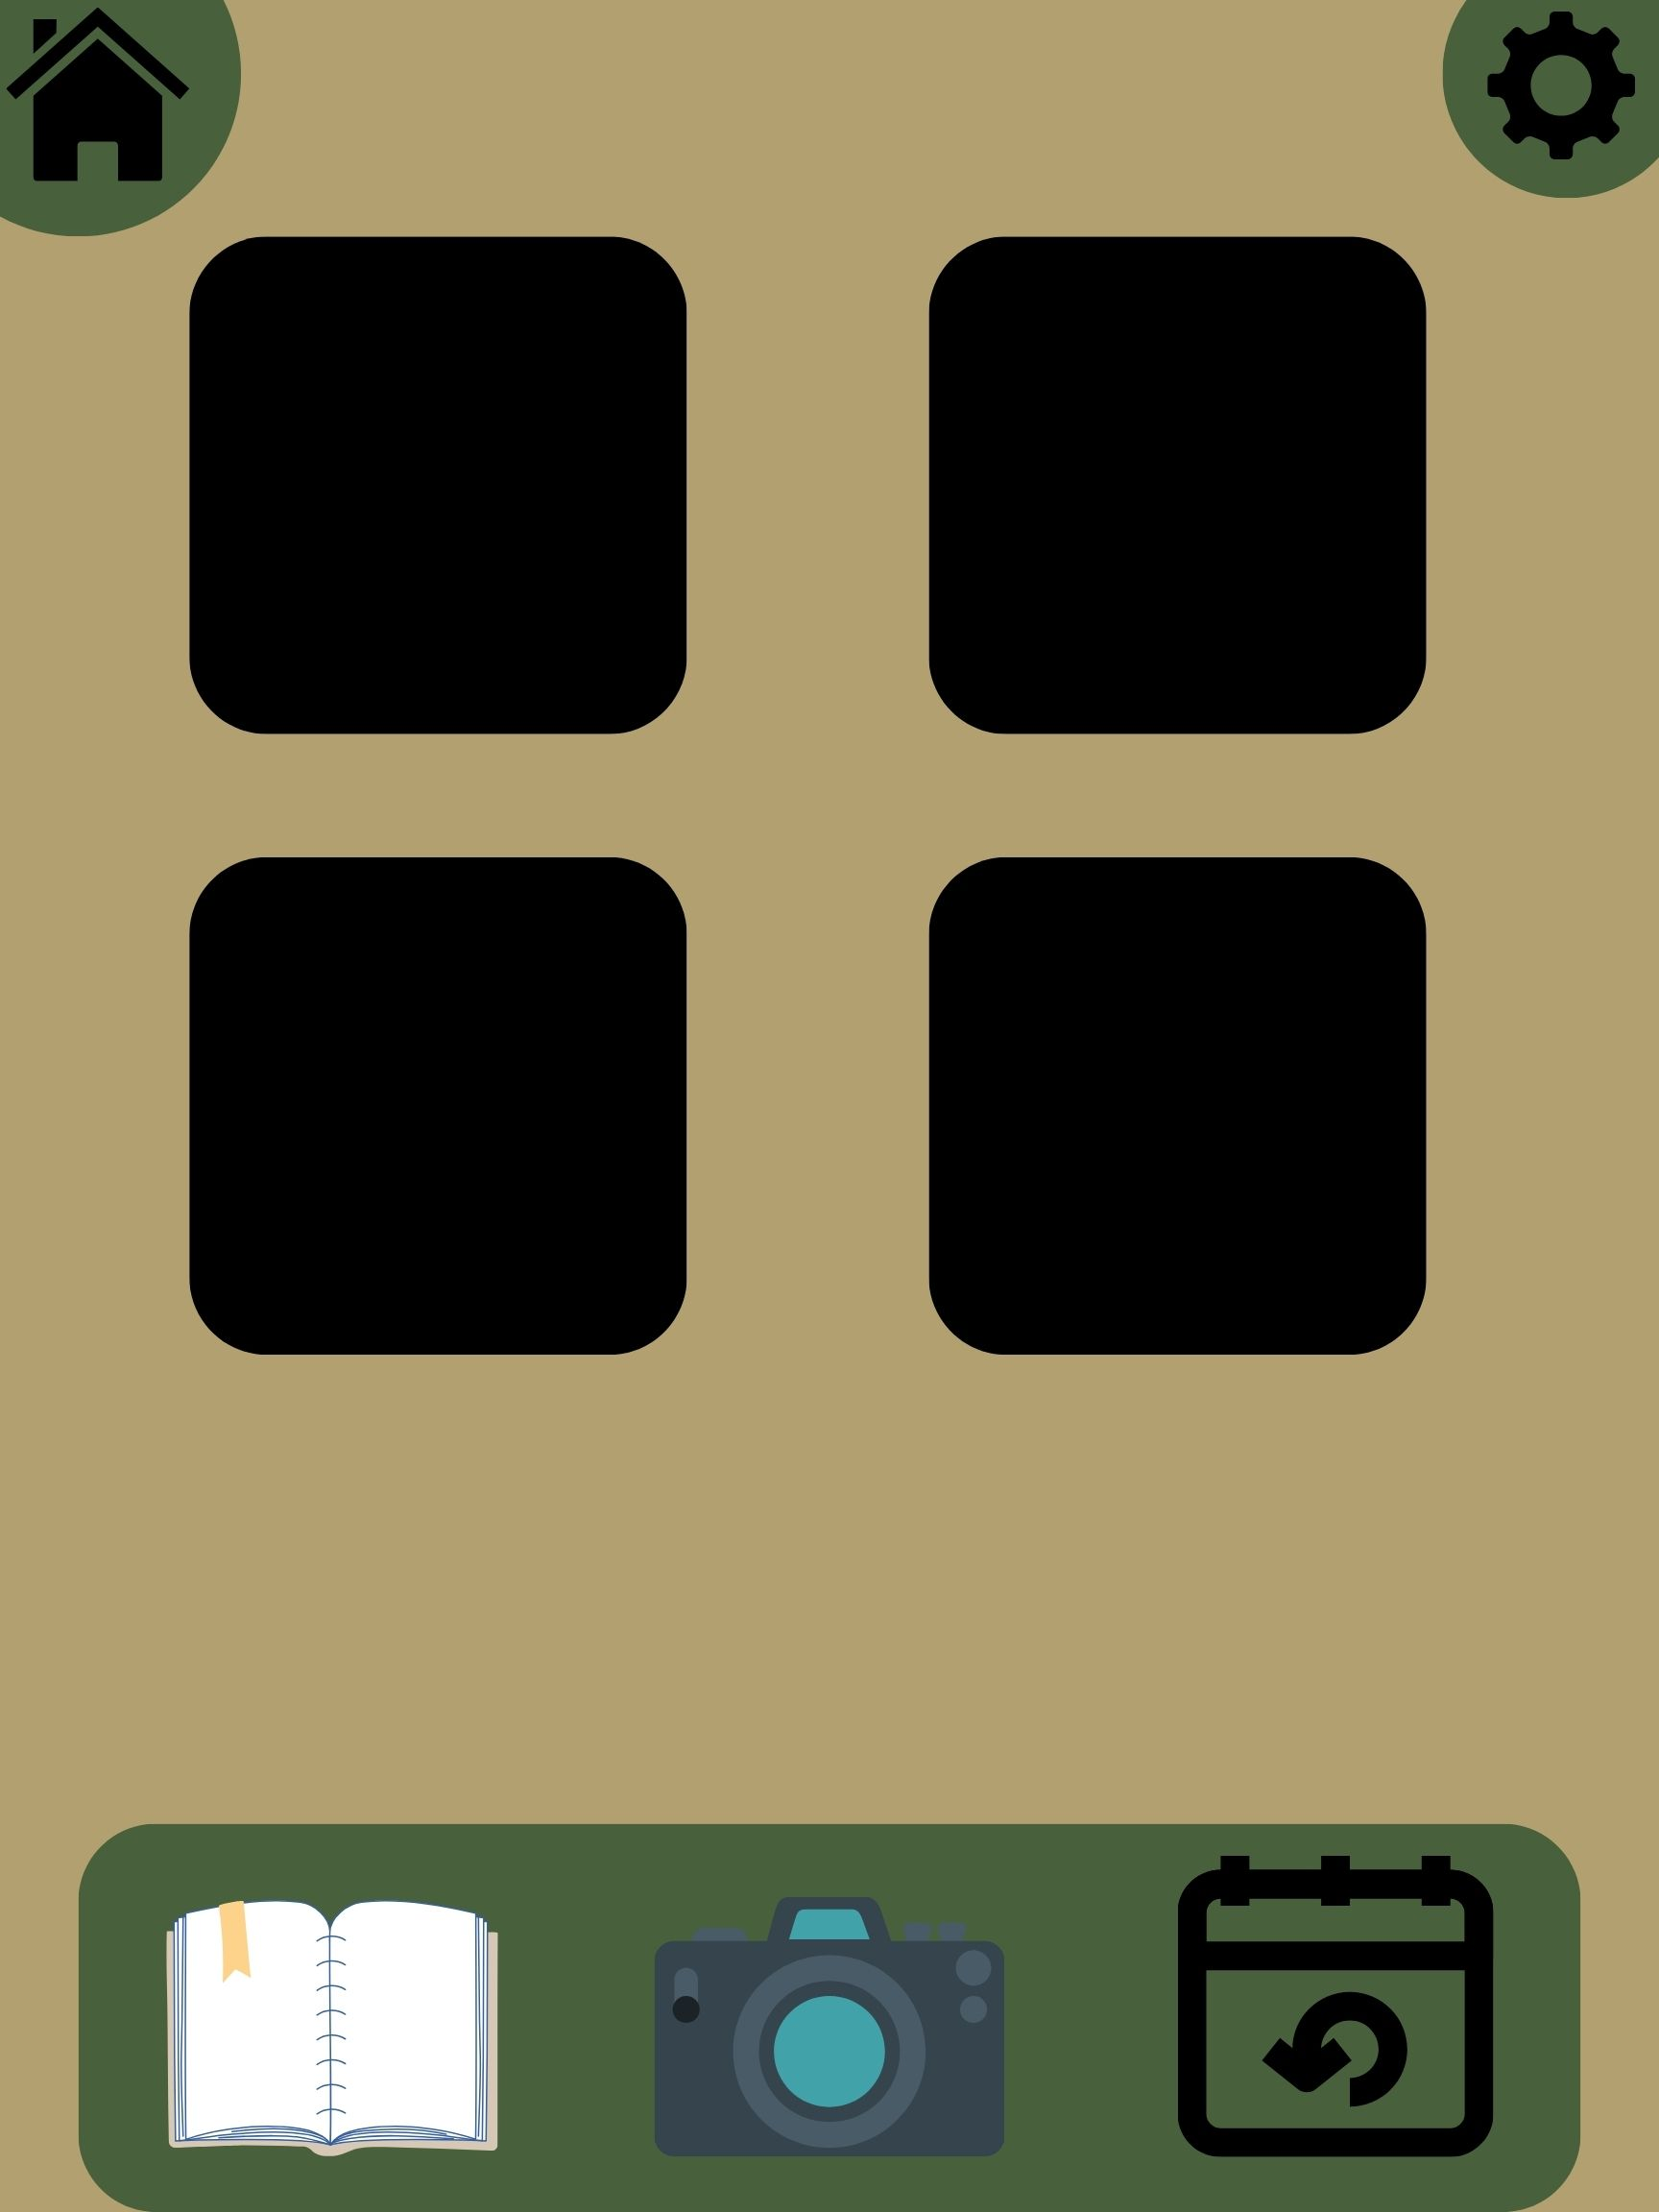
\includegraphics[width=2.5cm, height=4cm]{AllPlants}
	\\\emph{Figure 4-5.} Editing new or existing plant page and all plants wihtin journal page.
\end{figure}


\begin{figure}[H]
    \centering
    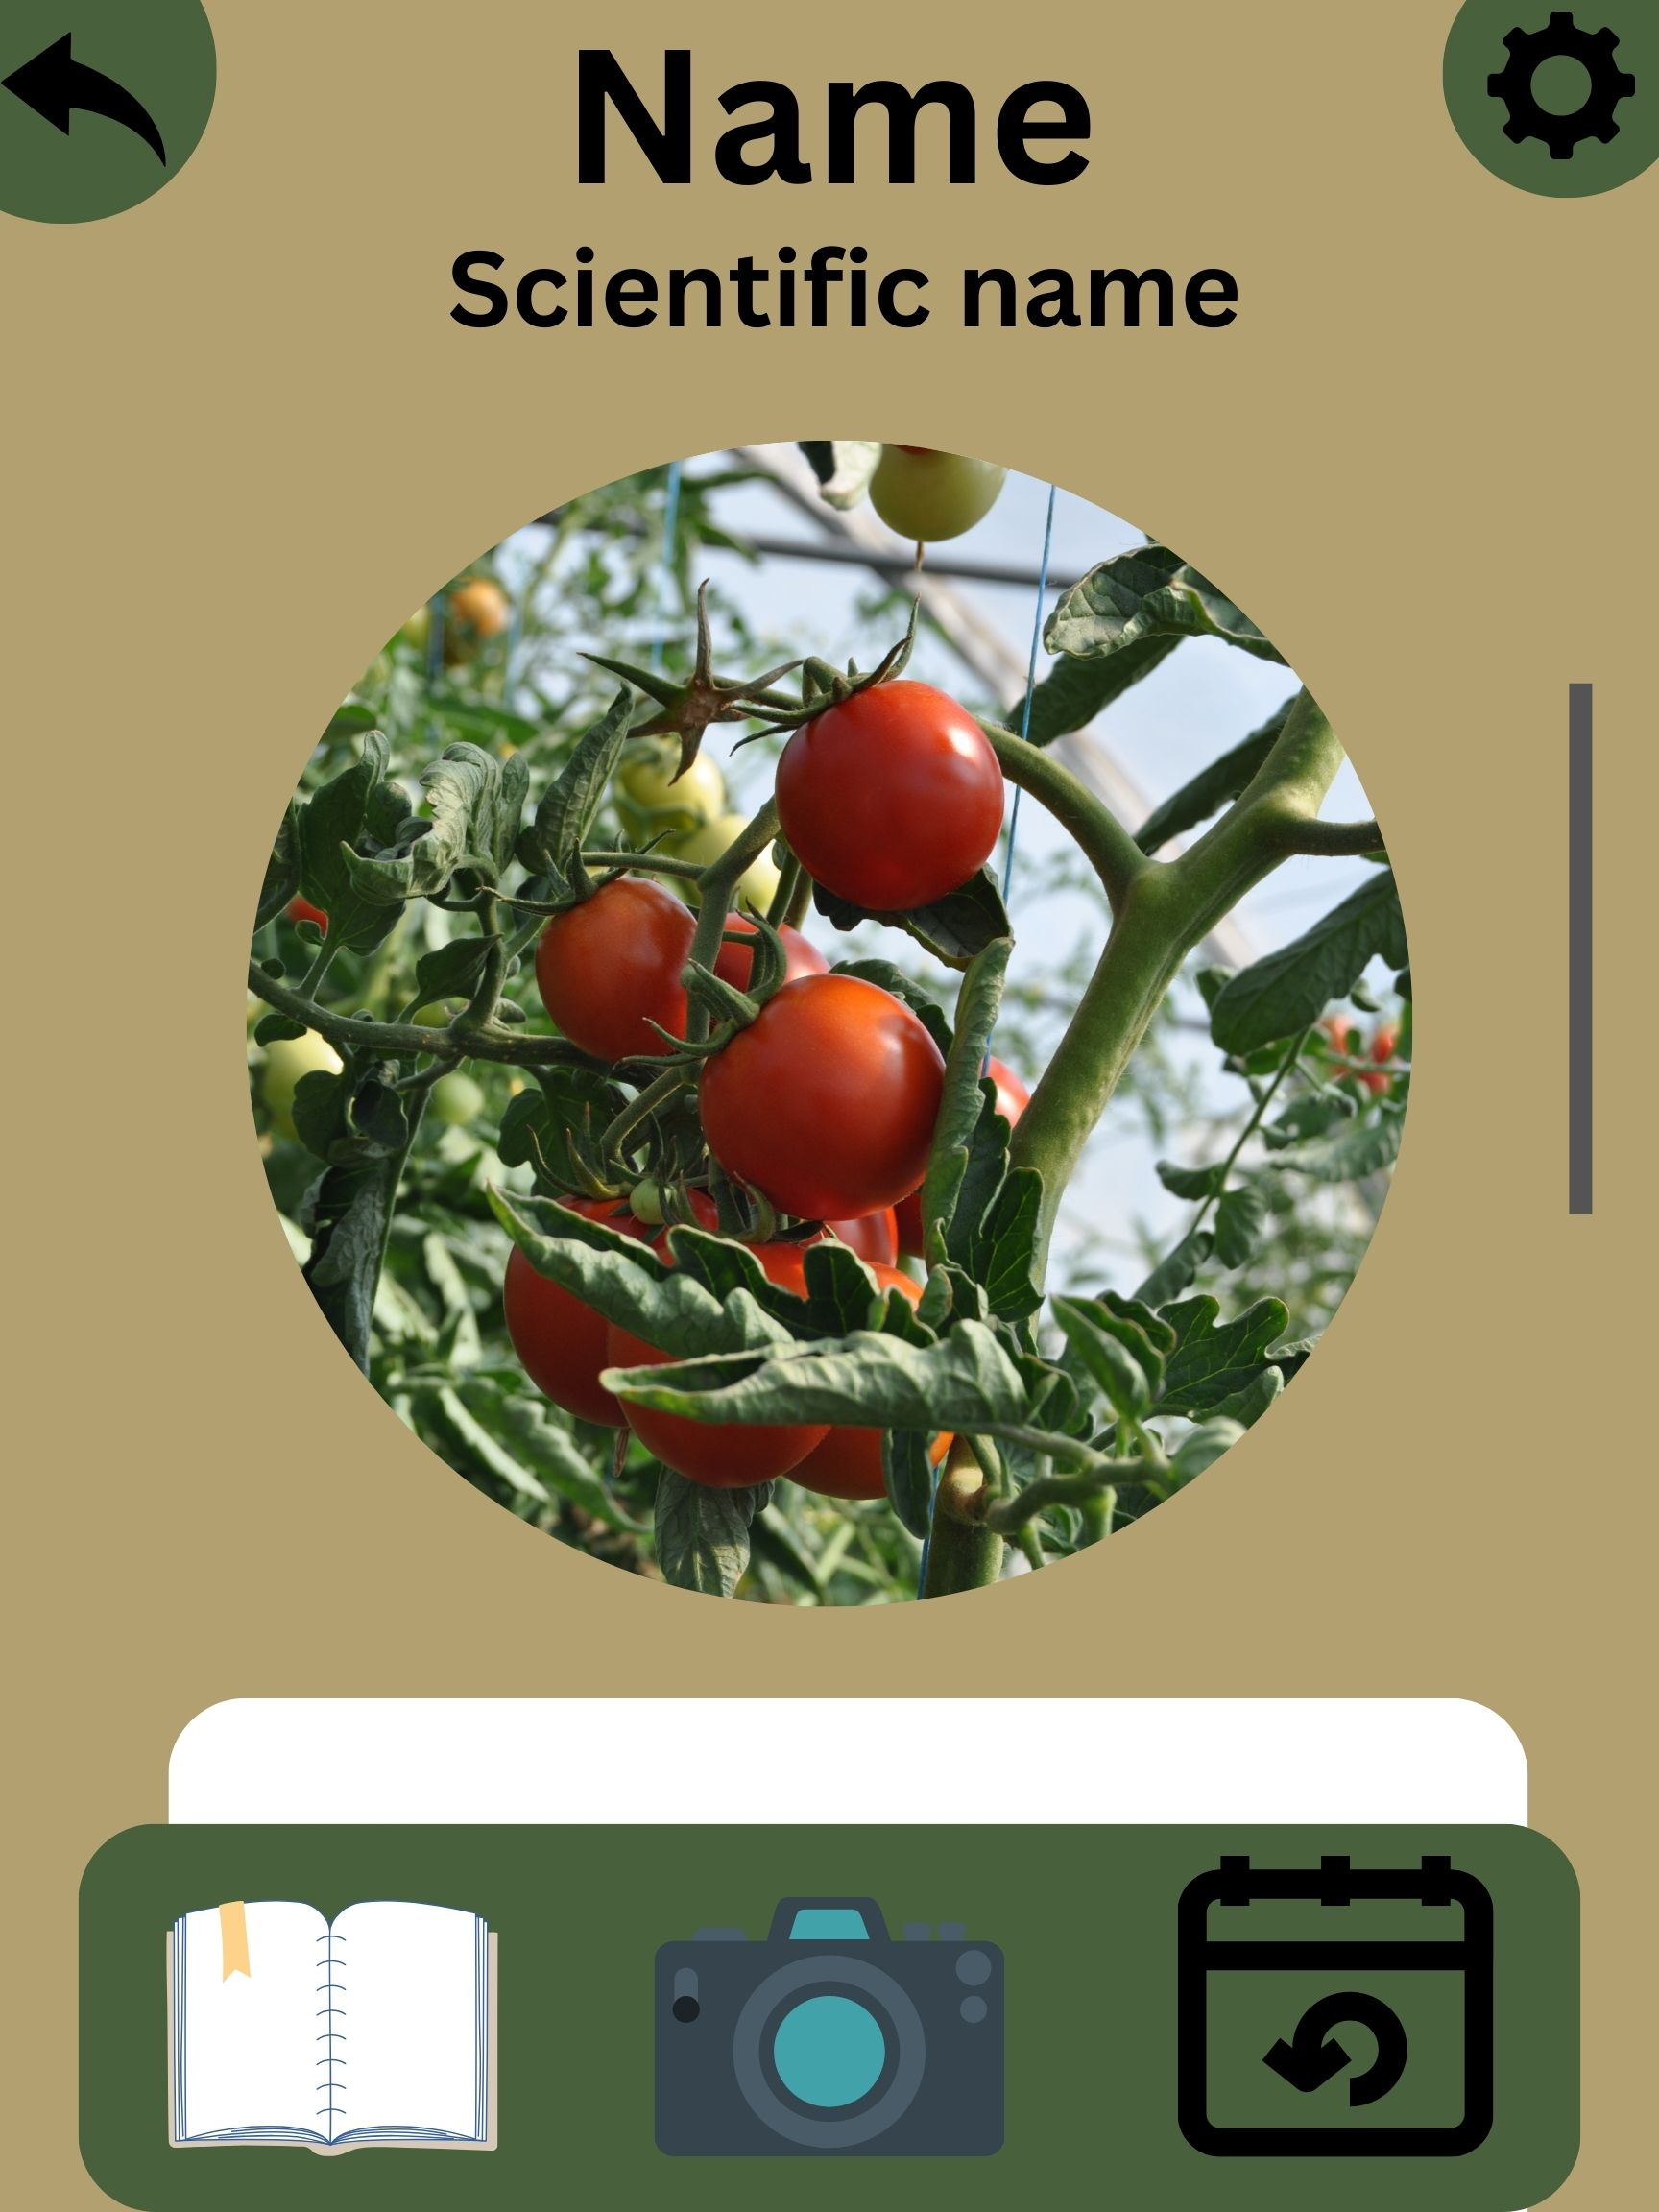
\includegraphics[width=2.5cm, height=4cm]{PlantClicked}
        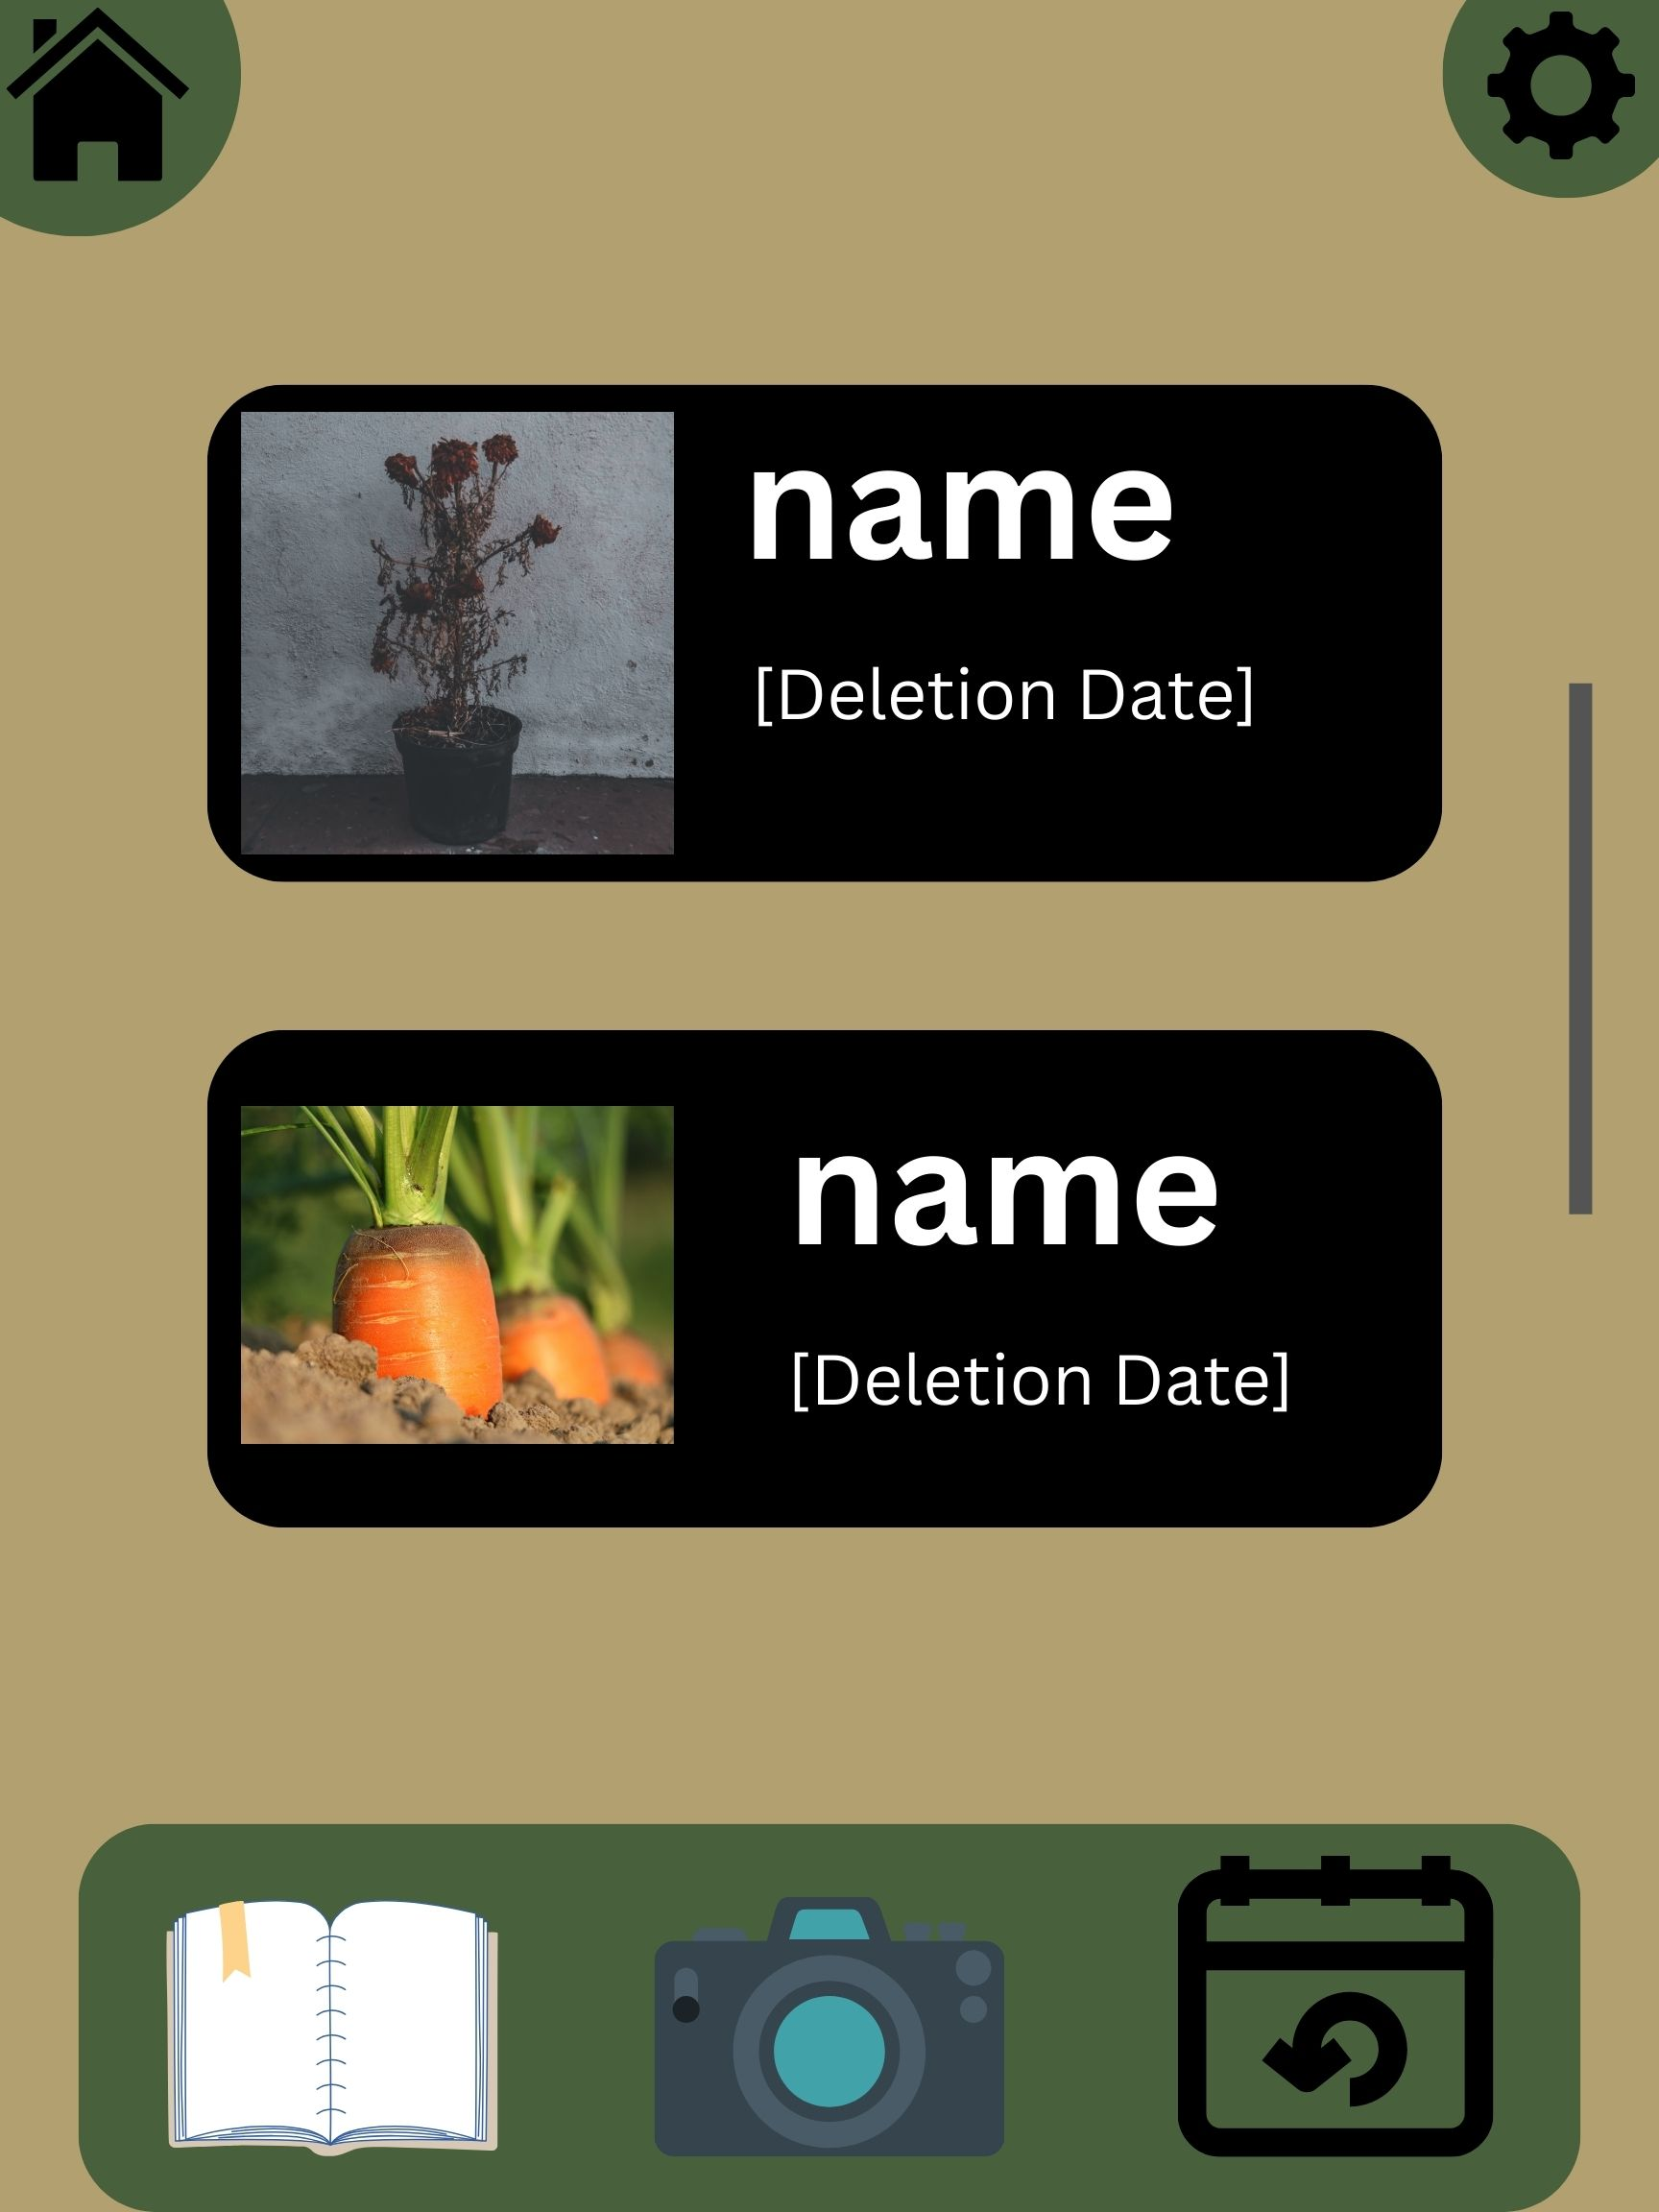
\includegraphics[width=2.5cm, height=4cm]{PlantHistory}
	\\\emph{Figure 6-7.} Journal of a single plant page and deleted plants page.
\end{figure}


\section{Impact}
We are hoping our application will have a positive influence on our environment and can help people take care of their gardens better. We hope users can have more flourishing gardens through the app keeping track of users plants and helping them to maintain a proper watering schedule with the least amount of plants been thrown out due to severe neglect. With the help of the Perenual API, we can provide additional information which can result in better planting and help users to provide necessary nutrition.

\section{Key Terminology}
The Perenual API not only introduces the users to additional insights about their plants, it also introduces them to a specialized agricultural vocabulary. To enhance the comprehension of the information provided by the API, it is highly beneficial for users to familiarize themselves with any potential new terms. The data retrieved by the API contains four distinct cycles that users might encounter. 

The first term is perennial. Perennial defines plants that persist for more than two years, typically flowering and producing seeds repeatedly during their life cycle. These plants often withstand seasonal changes, regenerating and blooming year after year, contributing to a longer and more sustained presence in a garden or natural environment. 

 The second term is annual. Annual refers to plants that complete their entire life cycle within a single growing season. These plants germinate, grow, flower, produce seeds, and die off within a year. Unlike perennials, annuals are known for having a short life cycle. A clear understanding of annuals aids users in strategizing and maintaining a garden that showcases a wide range of changing blooms throughout the year.

The next term is biennial. Biennial refers to plants that take two years to complete their life cycle. In the first year, they grow leaves and stems. In the second year, they flower, produce seeds, and finish their life cycle before dying off. The seeds biennial plants produce may be the start of new plants, but there is no guarantee.

Lastly, the user may encounter the term biannual. Biannual refers to plants that complete their life cycle every two years. This term is less common than the previously discussed ones, and it signifies a unique growth pattern where the plant goes through all stages of its life cycle biennially. Biannual plants might germinate, grow, flower, produce seeds, and complete their life cycle every two years.

Understanding the distinctions among perennial, annual, biennial, and biannual plants is crucial for users harnessing the potential of the Perenual API. By familiarizing themselves with this specialized agricultural vocabulary, users are able to enhance their experience with the app.

\section{Audience}
The reader should have an understanding of Gardener's Best Friend's target audience so that the report can best understand the app and why it was designed. The app is aimed towards the average person who wish to take care of a garden of plants, but may not be able to properly track and care for each and every plant to the best of their ability. Gardener's Best Friend allows the audience to improve their plant-taking abilities by allowing the user to keep a diary of their plant by writing any actions the user performed that day or any inconsistencies that the user noticed. The app also provides the user information about each plant that allows each user to make adjustments to their usual plant-taking activities that can benefit each plant.


\section{Use Cases}
These are the use cases for the app. The table containing each ID can be found at Table \ref{tab:use_cases}.
\begin{table}[]
    \centering
    \begin{tabular}{|c|c|}
        \hline
         Name & Primary Actor \\
         \hline
         \hline
         1 & Open Add Plant Page\\
         \hline
         2 & Select Plant Image Using Camera \\
         \hline
         3 & Select Plant Image Using Existing Photo \\
         \hline
         4 & Add/Edit Weekly Reminders \\
         \hline
         5 & Add Journal Entry Date \\
         \hline
         6 & Add Journal Entry \\
         \hline
         7 & Confirm New Journal Entry \\
         \hline
         8 & View Home Screen \\
         \hline
         9 & View Current Plants \\
         \hline
         10 & View Specific Plant \\
         \hline
         11 & Edit Plant/Add New Entry \\
         \hline
         12 & View Plant History \\
         \hline
    \end{tabular}
    \caption{Plant Use Case IDs}
    \label{tab:use_cases}
\end{table}


%%\begin{itemize}
%%    \item Use Case ID: 1
%%    \item Actor: User
%%    \item Description: User wants to add a plant to the journal
%%    \item Precondition:
%%\begin{enumerate}
%%    \item The user must be at the home screen
%%\end{enumerate}
%%    \item Scenario: The user presses the "Add Plant" button, which is a leaf with a plus next to it
%%    \item Result: The system opens the add plant page
%%\end{itemize}

Use Case ID: 1
Actor: User \\
Description: User wants to add a plant to the journal \\
Precondition: The user must be at the Home screen \\
Scenario: The user presses the "Add Plant" button, which is a leaf with a plus next to it \\
Result: The system opens the add plant page \\
\\

Use Case ID: 2 \\
Actor: User \\
Description: User wants to add an image of their plant using the camera \\
Preconditions: \begin{itemize}
    \item The user must have given the app permission to use the camera
    \item The user must be on the add plant or edit plant screens
\end{itemize}
Scenario: \begin{enumerate}
    \item The user presses the large image frame at the top of the screen below the "Confirm" button
    \item The user presses the button labeled "Use Camera"
    \item The user takes a picture of their plant using the camera
\end{enumerate}
%%The user presses the large image frame at the top of the screen below the "Confirm" button. The user then presses the button labeled "Use Camera". The user then takes a picture of their plant using the camera. \\
Result: The picture taken by the user is displayed on the image frame that the user pressed \\
\\

Use Case ID: 3 \\
Actor: User \\
Description: Use wants to add an image of their plant using a existing photo in their gallery \\
Preconditions: \begin{itemize}
    \item The user must have given the app permission to view their images
    \item The user must be on the add plant or edit plant screens
\end{itemize}
Scenario: \begin{enumerate}
    \item The user presses the large image frame at the top of the screen below the "Confirm" button
    \item The user persses the button labeled "Use Gallery"
    \item The user selects an image of their plant from the photo gallery
\end{enumerate}
Result: The picture selected by the user is displayed on the image frame that the user pressed \\
\\

Use Case ID: 4 \\
Actor: User \\
Description: The user wants to add or edit the weekly reminders of their plant \\
Precondition: The user must be on the add plant or edit plant screens \\
Scenario: \begin{enumerate}
    \item The user presses the field labeled "Reminders (Optional)"
    \item The user selects the days they want to get reminders for their plant
\end{enumerate}
Result: The user's new reminders are selected \\
\\

Use Case ID: 5 \\
Actor: User \\
Description: The user wants to add a date to their plant's journal entry \\
Precondition: The user must be on the add plant or edit plant screens \\
Scenario: \begin{enumerate}
    \item The user selects the field above the Journal Entry field, which contains the required date format
    \item The user enters the date of their journal entry in the specified date format
\end{enumerate}
Result: The user's journal date is entered \\
\\

Use Case ID: 6 \\
Actor: User \\
Description: The user wants to enter a journal entry for their plant \\
Precondition: The user must be on the add plant or edit plant screens \\
Scenario: \begin{enumerate}
    \item The user selects the large field labeled "Write your diary entry..."
    \item The user enters the journal entry for the plant
\end{enumerate}
Result: The user's journal entry is entered \\
\\

Use Case ID: 7 \\
Actor: User \\
Description: The user wants to confirm their new plant or their new journal entry \\
Preconditions: \begin{itemize}
    \item The user must be on the add plant or edit plant screens 
    \item The user must have provided an image and entered a journal entry date and a journal entry
\end{itemize}
Scenario: The user presses the button labeled "Confirm" \\
Result: The user's new plant is added or their new journal entry is entered and the user is at the Home screen \\
\\

Use Case ID: 8 \\
Actor: User \\
Description: The user wants to go to the home screen \\
Precondition: The user must be on the My Diary or History screens \\
Scenario: The user presses the left menu button at the bottom of the screen, which is a globe with leaves \\
Result: The user is at the home screen

Use Case ID: 9 \\
Actor: User \\
Description: The user wants to view their current plants by accessing the My Diary screen \\
Precondition: The user must be on the Home or History screens \\
Scenario: The user presses the middle menu button at the bottom of the screen, which is a diary with a pencil \\
Result: The user is on the My Diary screen and all added plants are shown \\
\\

Use Case ID: 10 \\
Actor: User \\
Description: The user wants to view a specific plant's page
Preconditions: \begin{itemize}
    \item The user must be on the My Diary screen
    \item The user must have added a plant
\end{itemize}
Scenario: The user presses the plant entry containing the plant they want to view \\
Result: The user is viewing the selected plant's page \\
\\

Use Case ID: 11 \\
Actor: User \\
Description: The user wants to edit their plant's reminders or add a new diary entry \\
Precondition: The user must be on the page of the plant they want to edit or add a new diary entry for \\
Scenario: The user presses the pencil icon at the bottom right of the plant's image \\
Result: The user is on the edit plant screen \\
\\

Use Case ID: 12 \\
Actor: User \\
Description: The user wants to view a history of their deleted plants \\
Precondition: The use must be on the Home or My Diary screens \\
Scenario: The user presses the bottom right menu button at the bottom of the screen, which is an hourglass timer containing a substance that looks like the Earth \\
Result: The user is at the History screen \\

\section{Challenges}
In the course of our project development, we encountered a myriad of challenges that required diligent problem-solving and creative solutions. One notable hurdle pertained to obtaining the necessary permissions for various functionalities, including camera usage, gallery access, and calendar integration. Navigating the intricate landscape of permissions proved to be a multifaceted task, demanding careful consideration of user privacy and security concerns.

Another noteworthy challenge we confronted revolved around the seamless implementation of reminders within our application. Ensuring that reminders occurred reliably and at the appropriate times presented a complex puzzle that demanded meticulous attention to detail and rigorous testing. This aspect of our development process underscored the importance of creating a user experience that not only met but exceeded expectations.

Additionally, our journey in the development realm brought us face to face with compatibility issues between SQLite and Java database. It became apparent that these two database systems posed a compatibility dilemma, requiring a thoughtful evaluation of our database architecture. Ultimately, We decided to cut Java database and use SQLite. The intricacies involved in resolving this issue highlighted the nuanced nature of database management and underscored the significance of choosing the right tools for the job.

In summary, our project's development path was marked by challenges that spanned permissions management, reminder functionality, and database compatibility. Each obstacle presented an opportunity for growth, learning, and ultimately, the enhancement of our application's overall quality and user experience.

\section{Results}
To wrap this application up, the bullets below are what we have fully working.
\begin{itemize}
    \item Journal
    \item Photo records
    \item Notification (Reminders for watering schedule)
    \item API for additional plant information
    \item Database
\end{itemize}

\section{Future Work}

In envisioning the future development of our plant care application, a compelling avenue for expansion lies in the incorporation of location-based services to enhance plant care recommendations. By integrating location services, we aim to seamlessly tie into weather forecasting applications, providing users with real-time and localized weather information pertinent to their geographical location. This innovative feature would empower users to make informed decisions about their plant care routines, aligning them with the specific climatic conditions influencing their plants.

The integration of location services could enable the application to dynamically adapt its recommendations based on factors such as temperature, humidity, and sunlight exposure unique to each user's region. For instance, users in colder climates might receive tailored suggestions during winter months, ensuring their plants receive adequate protection and care against frost. Conversely, users in warmer climates may receive guidance on managing hydration levels during hot summer days.

Furthermore, this feature could facilitate the automatic adjustment of watering schedules and other care routines, creating a personalized and responsive experience. By tapping into real-time weather data, the application could provide timely alerts or notifications, prompting users to take proactive measures in response to sudden weather changes.

Incorporating location-based weather services not only elevates the sophistication of our plant care application but also aligns with our commitment to delivering a holistic and user-centric experience. As we look toward the future, this expansion into dynamic, location-aware plant care features holds the potential to redefine the way users interact with and care for their plants, fostering a more intuitive and adaptive connection between technology and nature.

\section{Conclusion}


In conclusion, this application stands as a sophisticated and user-centric solution for plant enthusiasts seeking a comprehensive tool to enhance their plant care experience. The diverse range of features, from the intuitive diary function to the seamless integration of visual elements through camera and gallery access, demonstrates a commitment to providing users with a personalized and enriching journey in plant maintenance.

The incorporation of the API introduces a layer of intelligence, offering users valuable insights into the scientific details of their plants. This not only educates users but elevates the app to a more dynamic and informative platform.

The calendar system,  leveraging the built-in calendar, reflects a thoughtful approach to user engagement. This feature ensures that users stay proactive in their plant care routines, with timely reminders for diary entries and essential activities like watering.

The forward-looking integration of location services adds a practical dimension, connecting users with real-time weather forecasts based on their geographical location. This not only underscores the app's commitment to informed decision-making but also reinforces its adaptability to the specific environmental conditions influencing plant health.

In essence, this application transcends the conventional boundaries of a plant diary, evolving into a multifaceted companion for plant enthusiasts. By amalgamating technological advancements, educational features, and user-friendly design, it not only meets but exceeds the expectations of users, fostering a deeper and more meaningful connection between individuals and their green companions.



% Balancing columns in a ref list is a bit of a pain because you
% either use a hack like flushend or balance, or manually insert
% a column break.  http://www.tex.ac.uk/cgi-bin/texfaq2html?label=balance
% multicols doesn't work because we're already in two-column mode,
% and flushend isn't awesome, so I choose balance.  See this
% for more info: http://cs.brown.edu/system/software/latex/doc/balance.pdf
%
% Note that in a perfect world balance wants to be in the first
% column of the last page.
%
% If balance doesn't work for you, you can remove that and
% hard-code a column break into the bbl file right before you
% submit:
%
% http://stackoverflow.com/questions/2149854/how-to-manually-equalize-columns-
% in-an-ieee-paper-if-using-bibtex
%
% Or, just remove \balance and give up on balancing the last page.
%
\balance{}

\section{References} 
\nocite{API2}
\nocite{API}
\nocite{Buttons}
\nocite{Notifications}
\nocite{Perenual}
\nocite{SQLITE}
\nocite{Freepik}
% REFERENCES FORMAT
% References must be the same font size as other body text.

%%\bibliographystyle{SIGCHI-Reference-Format}
%%\bibliographystyle{acm-sigchi-proceedings}
\printbibliography
\end{document}


